\subsection{UC13 - Verifica dello stato di \glossario{Check-in}/Check-out}
\begin{itemize}
	\item \textbf{Identificativo}: UC13
	\item \textbf{Nome}: Verifica dello stato di \glossario{Check-in}/Check-out
	\item\textbf{Descrizione Grafica}: 
	\begin{center}
		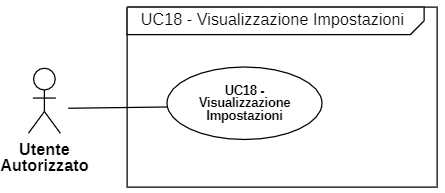
\includegraphics[scale=0.65]{images/UC13.png} 
	\end{center}

	\item \textbf{Attori}
	\begin{itemize} 
		\item \textit{Primari}: Utente autorizzato
		\item \textit{Secondari}: Non presenti
	\end{itemize}
	\item \textbf{Descrizione}: L'utente richiede conferma sull'attuale stato di \glossario{Check-in}/Check-out.
	\item \textbf{Precondizione}: L'utente ha effettuato il login e si trova nella chat.
	\item \textbf{Postcondizione}: Chatbot restituisce l'attuale stato di Check-in/Check-out.
	\item \textbf{Scenario principale}:  \begin{enumerate}
		\item Utente invia un messaggio del tipo : "Ho eseguito il check-in?";
		\item Chatbot risponde restituendo i Check-in/Check-out effettuati nella stessa data.
	\end{enumerate}
\end{itemize}